%%%%%%%%%%%%%%%%%%%%%%%%%%%
%                                                          %
%                          Experiment M-6                  %
%          Ballistic Pendulum & Projectile Motion          %
%                                                          %
%%%%%%%%%%%%%%%%%%%%%%%%%%%

%\labChapter{M}{The Ballistic Pendulum and Projectile Motion}
\labChapter{M}{Conservation of Energy \& Linear Momentum with Ballistic Pendulum \& Projectile Motion}
\label{lab:M6}

% Introduction
%\section{Introduction}
% Background
\section{Background}

Conservation of energy and linear momentum will be used to measure the initial velocity of a projectile.  Two techniques will be employed.

In the first, a ballistic pendulum, a device designed to capture a projectile in an initially stationary pendulum, will be used.  The conservation principles are used to analyze the collision and the subsequent motion of the pendulum.  The completely inelastic collision associated with the capture of the projectile in the pendulum and the subsequent motion of the pendulum provide the data necessary for the determination of the initial velocity.

In the second technique, the measured parameters of the trajectory of a horizontally launched projectile are used to determine the initial velocity.  With the projectile moving in a free-fall trajectory, constant acceleration kinematics will be used to determine the initial velocity from measurements of the horizontal range and vertical drop.

In each case, the projectile will be launched with the same device allowing a comparison of the initial velocity determinations of the two techniques.




% Ballistic Pendulum
\subsection{Ballistic Pendulum}

The ballistic pendulum is so named because it was originally used to measure the velocity of high-speed projectiles such as bullets long before electric and electronic timers made the procedure unnecessary.  It remains, however, as a simple and demonstrative device for understanding the conservation principles of energy and momentum.  In analyzing the problem, the system will consist of the projectile and the more massive pendulum.  As illustrated in the left image in Fig.~\ref{M06Fig01}, before the collision, the projectile is in motion horizontally towards the stationary pendulum.  After the collision, the projectile is imbedded in the pendulum and the pendulum is moving along the arc as shown in the right image of Fig.~\ref{M06Fig01}.

\begin{figure}
  \begin{center}
    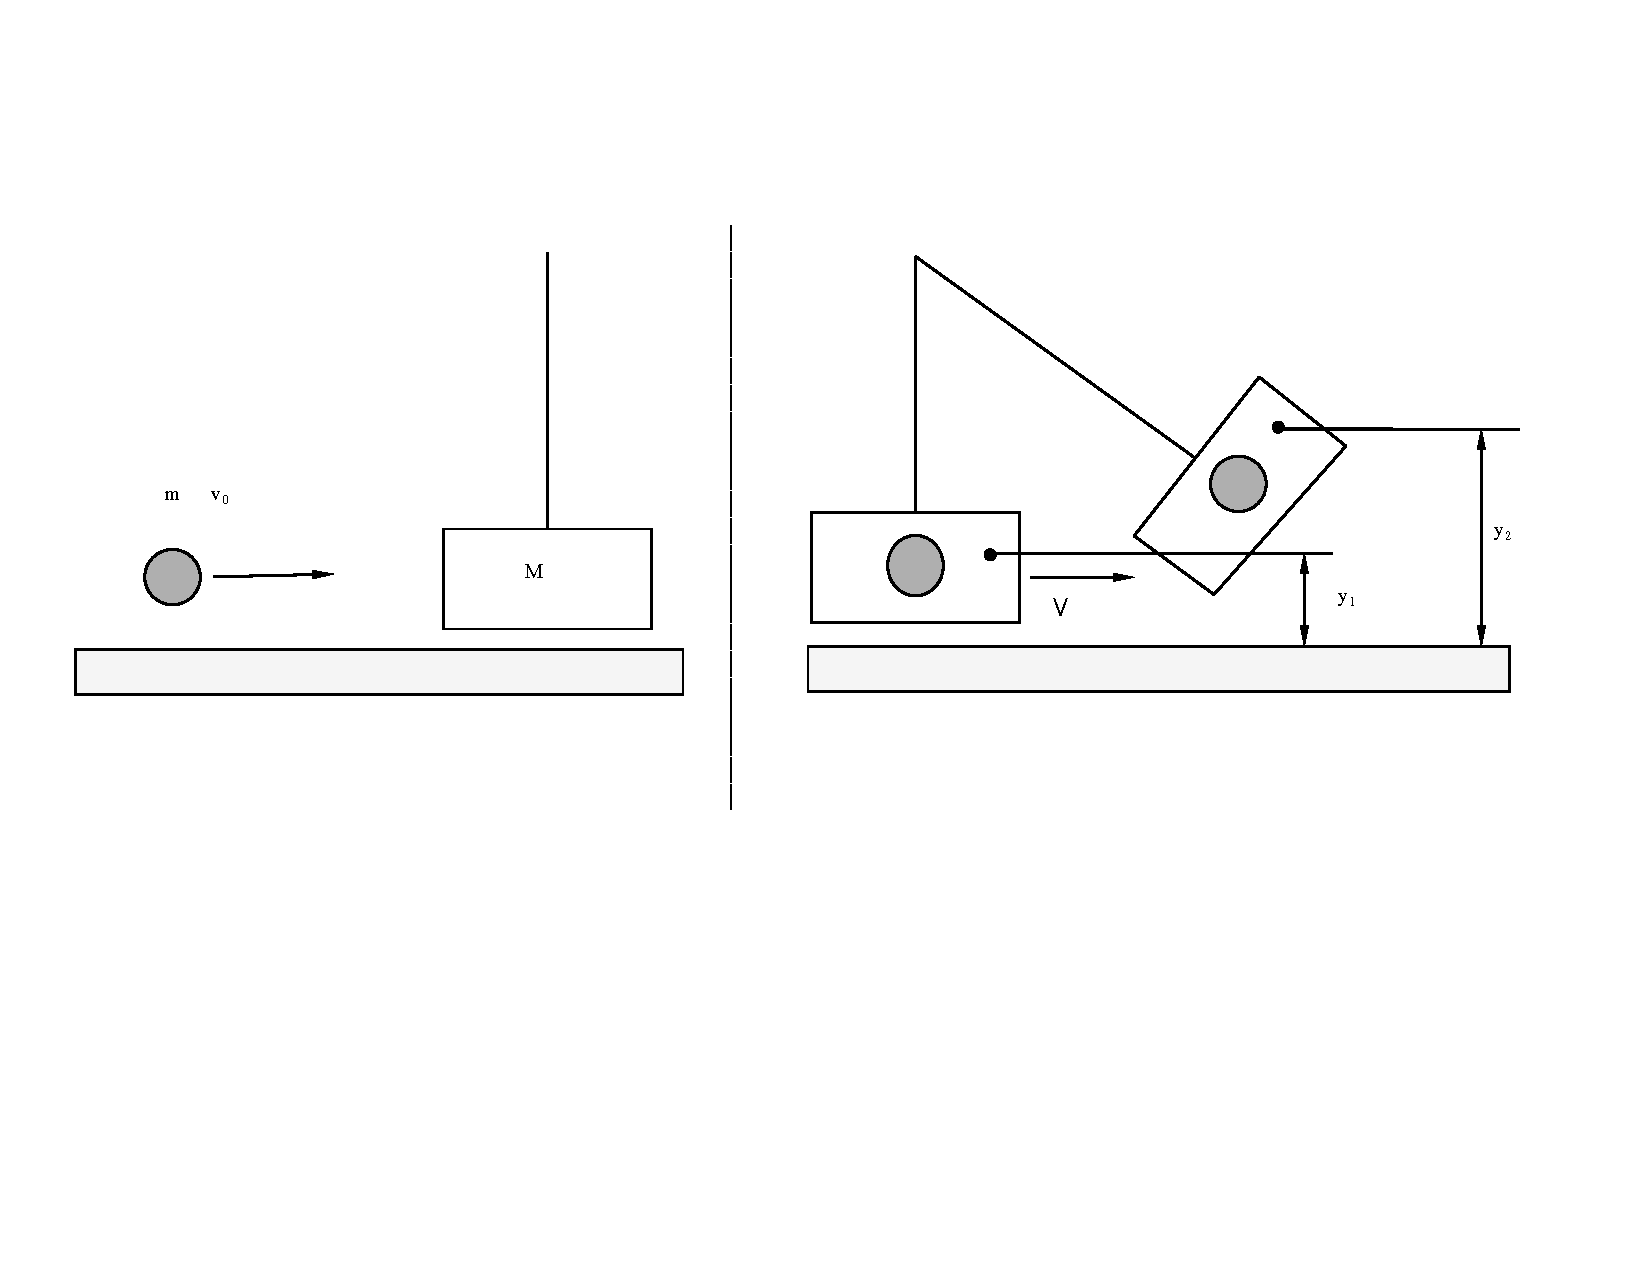
\includegraphics[width=5in]{Experiment05Figures/Figure01a.pdf}
  \end{center}
  \caption{Ballistic Pendulum before (left) and after the collision (right)}
  \label{M06Fig01}  % the \label command comes AFTER the caption
\end{figure}

The horizontally launched brass ball collides rather violently with and is captured by the more massive bob of the pendulum, initially at rest.  The violent collision is totally inelastic as the ball is captured by the pendulum with much of the initial kinetic energy of the ball lost through a variety of energy conversions, mostly heat.

During the collision of the ball with the pendulum, no external forces are acting on the system.  Newton's third law demands that the forces of the ball on the pendulum and the pendulum on the ball are equal and opposite.  These two, always equal and opposite, internal forces are acting for the same time and therefore produce equal and opposite impulses on the two bodies. Thus the change in momentum of one body is equal and opposite to the change in momentum of the other.  If the momentum changes of the two colliding bodies are equal and opposite, then the total linear momentum of the system cannot change and the total momentum is conserved.

Notice that there has been no assumption on the nature of the internal forces acting.  They do not have to be elastic, i.e.\ conservative.  As such, the conservation of momentum does not imply anything about the conservation of kinetic energy in the collision.  Linear momentum is conserved regardless of the nature of the interaction of the two bodies during the collision.  Only when the interactive forces are completely elastic, i.e.\ conservative, will the kinetic energy of the collision be conserved.

Momentum, like force and velocity, is a vector quantity.  The conservation of momentum of a system therefore implies the conservation of the total vector momentum of the system.  In our case, the initial momentum of the system is the initial momentum of the brass ball, which is only in the horizontal direction.  Therefore the momentum after the collision can only be in the horizontal direction and they must be equal.

Thus we can write
\begin{equation}
  \label{eq:M06momentum}
  m \vec{v}_0 = (m + M) \vec{V},
\end{equation}
where $m$ is the mass of the ball, $M$ is the mass of the pendulum, and $\vec{V}$ is the velocity of the pendulum and ball together.  If we can measure or determine $\vec{V}$, we can determine $\vec{v}_0$.  The determination of $\vec{V}$ can be made by examining the motion of the pendulum after the collision.

After the collision, the pendulum swings upward until it momentarily comes to rest at the top of its swing where the vertical height of the system has been increased from $y_1$ to $y_2$ (right image of Fig.~\ref{M06Fig01}).  We will now make some assumptions.  We will assume that there are no friction losses in the motion of the pendulum and that no collisions take place that might otherwise cause a loss of mechanical energy.  In other words, we are assuming that the total mechanical energy of the system is conserved after the collision.  By equating the kinetic energy of the system just after the collision at the bottom of the swing to the potential energy at the top, we can write
\[
\frac{1}{2}(m+M) V^2 = (m+M)  g \left(y_2 - y_1\right).
\]
Solving this expression for $V$ we have
\[
V = \sqrt{2 g \left(y_2 - y_1\right)}.
\]

Substituting in Eqn.~\ref{eq:M06momentum} above, we have finally an expression for the initial velocity of the ball in terms of the measurable change in height of the pendulum and the respective masses, i.e.
\begin{equation}
  \label{eq:M06v0} 
  v_0 = \left( \frac{m+M}{m} \right) \sqrt{2 g \left(y_2 - y_1\right)}.
\end{equation}

% Projectile Motion
\subsection{Projectile Motion}

When a projectile is moving solely under the influence of the force of gravity, we say that the projectile is in free-fall.  Consider the launching of the same ball used in the ballistic pendulum.  In this case, the pendulum will be swung up out of the way so the flight of the ball will continue off the edge of the table, eventually hitting the floor some distance away.  This situation is illustrated in Fig.~\ref{M06Fig02}.

\begin{figure}
  \begin{center}
    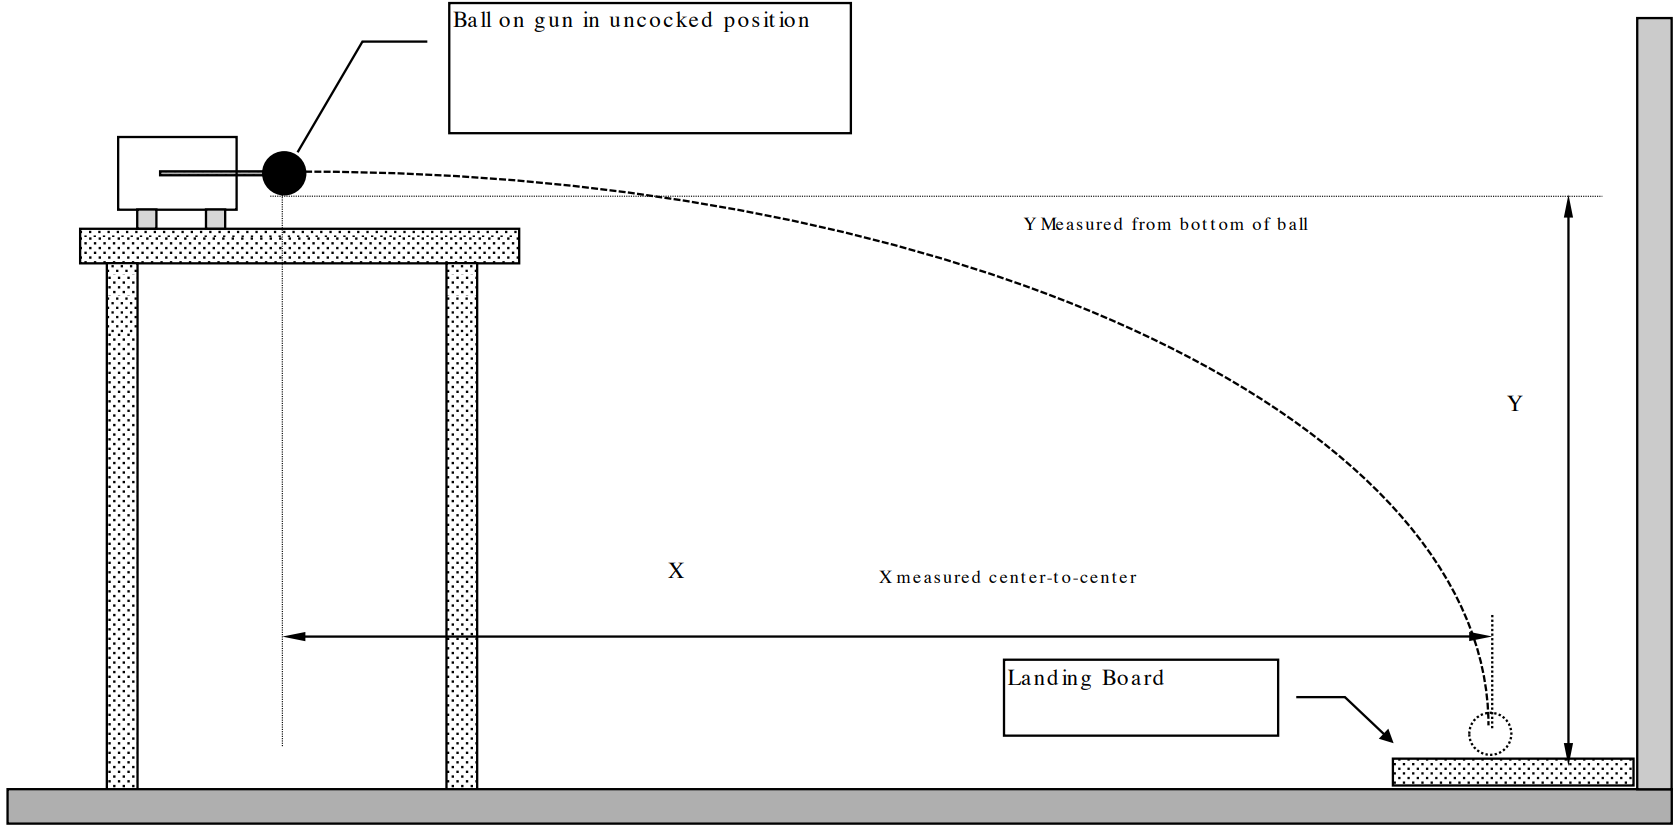
\includegraphics[width=6in]{Fall/Experiment05Figures/M06_fig02.png}
  \end{center}
  \caption{Projectile Motion}
  \label{M06Fig02}
\end{figure}

Once the ball leaves the spring gun used to launch the ball, the ball is in free-fall.  The vertical and horizontal motions are completely independent.  We assume that once the ball leaves the gun, there are no energy loss mechanisms during the flight of the ball.

In the vertical direction, the initial velocity is zero and the ball is accelerated downward by its weight, finally hitting the floor some time, $t$, later, dropping a vertical distance of $Y$.
In the horizontal direction, the ball has a constant velocity of $v_0$ during the entire flight over the horizontal distance $X$.

Using our kinematic expressions for constant acceleration motion, we have
\[
Y = \frac{1}{2} g t^2
\]
and
\[
X = v_0 \, t.
\]
Eliminating the time $t$ from these two expressions, we obtain
\begin{equation}
  \label{eq:M06v0pro}
  v_0 = X \sqrt{\frac{g}{2 Y}}.
\end{equation}


\section{Experimental Procedure}

% Ballistic Pendulum
\subsection{Ballistic Pendulum}

\begin{enumerate}
\item Data table:
\begin{itemize}
\item Create a table of the common data for the ballistic pendulum experiment including the mass of the ball $m$, the mass of the pendulum $M$, the initial pendulum height $y_1$ and any other common data needed for calculations.
\item Create a table with a row for each of the ten trials in the ballistic pendulum part of this lab including the trial number, %the rack number, 
the pendulum height $y_2$, the change in height $y_2-y_1$, the calculated velocity of the pendulum $V$, and the calculated initial velocity of the ball $v_0$.
\item Create a table to summarize the ten trials including the average pendulum height $y_2$, the average change in height $y_2-y_1$, the average velocity of the pendulum $V$, the average initial velocity of the ball $v_0$, the standard deviation of $v_0$.% and the standard deviation of the mean of $v_0$ using the methods in the Error Analysis section Eqns.~\ref{eq:errorSigmaX} and~\ref{eq:errorSigmaMeanX}.
\end{itemize}
\item Measure and record the mass of the brass ball projectile.
\item Record the mass of the pendulum that is indicated on the apparatus.
\item Practice the following procedure before actually taking data.
\item The pointer on the side of the bob indicates the center of mass of the pendulum.  With the pendulum hanging motionless, measure the height above the base plate of the pointer.  This value is $y_1$.   Record the value in meters.
\item Place the brass ball on the pin of the gun and press the ball so the spring of the gun is compressed until the trigger catches and holds the compressed spring.
\item Fire the gun by squeezing the trigger.  The ball will be captured by the bob and the pendulum will swing upwards.
\item A small ratchet engaging a rack will capture the maximum upswing position of the pendulum. % Note the value on the side of rack where the bob comes to rest and 
Measure the height to the tip of the metal pointer on the pendulum which represents the center of mass of the pendulum with ball.
\item Carefully release the ratchet so the pendulum can swing back to its equilibrium position.
\item Release the ball from the bob of the pendulum by pushing it with your finger or a short cylinder.  
\item Fire the ball ten times, and record the %rack number and 
pendulum height $y_2$ for each shot.
\item Calculate the average $y = y_2-y_1$ and the average $v_0$ from Eqn.~\ref{eq:M06v0}.
%\item Using the calculus method and assuming the error in $v_0$ comes from the variation in $y_2$, calculate the standard deviation
%  \begin{equation}
%    \label{eq:M06StandardDev}
%    \sigma(v_0) = \left(\frac{1}{2}\right)\frac{\bar{v}_0\, \sigma(y_2)}{\bar{y}_2 - y_1}.
%  \end{equation}
\item Record your data and calculations on your spreadsheet.
%\item You have multiple measurements that each give $v_0$. The average value is more precise than any individual measurement. The standard deviation of the mean value is less that the standard deviation of individual measurements. See Eqn.~\ref{eq:errorSigmaMeanX}. Your estimate of the error of the average of $n=10$ measurements is $\sigma(\bar{v}_0) = \sigma(v_0)/\sqrt{n-1}$ where $n=10$ is the number of measurements.


\end{enumerate}



% Projectile Motion
\subsection{Projectile Motion}

\begin{enumerate}
\item Data table:
\begin{itemize}
\item Create a table of the common data for the projectile motion experiment including the distance to the pad $x_1$, the vertical distance $Y$ and any other measurements.
\item Create a table with a row for each of the ten trials in the projectile motion part of this lab including the trial number, the measured $x_2$, the calculated horizontal distance $X=x_1+x_2$ and the calculated initial velocity of the ball $v_0$.
\item Create a table to summarize the ten trials including the average initial velocity $v_0$ of the ball, the standard deviation of $v_0$.% and the standard deviation of the mean of $v_0$.
\end{itemize}
\item Set up the projectile motion experiment as shown in Fig.~\ref{M06Fig02}.
\item Perform $n=10$ measurements of $x_2$. Be careful that the gun is in the same position for each measurement
\item Calculate the standard deviation for the $n=10$ measurements of $x_2$.
%\item Calculate the standard deviation for the velocity using the calculus method:
%\[
%  \sigma(v_0) = \bar{v}_0 \,\sigma(X) / \bar{X}
%\]
%where a bar over a symbol, as in $\bar{X}$, means the average value.
%\item Calculate the standard deviation of the mean of $v_0$.
\end{enumerate}



%\subsection{Comparing Projectile Motion and Ballistic Pendulum}
%The more measurements you make of a quantity, the better your estimate of the average value. The standard deviation of the mean is
%\[ \sigma(\bar{v}_0) = \frac{\sigma(v_0)}{\sqrt{n-1}}.\]
%Compare $\sigma(\bar{v}_0)$ from the projectile method and from the ballistic pendulum.  Which is larger? How do these numbers compare with the difference between $\bar{v}_0$ from the pendulum calculation and from the projectile calculation. If the difference of the two measurements is much larger than the standard deviation of the mean then you should suspect some systematic error. One possible systematic errors is an error in one of the other quantities which you measured only once. Another source of systematic error is some property of the apparatus that is not quite what you assumed.  What are some of the possible sources of systematic error in the two measurements?



\pagebreak

\section{Post-Lab Submission --- Interpretation of Results}

\begin{itemize}
    \item Make sure to submit your finalized data table (Excel sheet)
    \item What is the range of your measurements for both pendulum and projectile? Do the initial velocities agree within the ranges when treating your standard deviations as your uncertainty of average values?
    \item How and why are they (or could be) different.
   % \item The two results you found for $v_i$ are supposed to be the same value, since you used the same launching mechanism. 
    \item Which of the two results for the value of $v_i$ do you trust more? Explain your answer using a Physics argument.
    \item Suppose you would have used a more massive marble in the projectile motion portion of the experiment. How would this affect your result? Explain your answer.
    \item What are the effects of measured uncertainties on your determined velocities?
    \item What are possible systematic errors for today's experiments?
\end{itemize}



%Compare your standard deviations from the projectile method and from the ballistic pendulum. Which is larger? How do these numbers compare with the difference between $\bar{v}_0$ from the pendulum calculation and from the projectile calculation.


%Effect of uncertainties on your result?

%Compare $\sigma(\bar{v}_0)$ from the projectile method and from the ballistic pendulum.  Which is larger? How do these numbers compare with the difference between $\bar{v}_0$ from the pendulum calculation and from the projectile calculation.

%If the difference of the two measurements is much larger than the standard deviation of the mean then you should suspect some systematic error. One possible systematic errors is an error in one of the other quantities which you measured only once. Another source of systematic error is some property of the apparatus that is not quite what you assumed.  What are some of the possible sources of systematic error in the two measurements?


